\section{Propuesta de solución}

Con la realización del proyecto que se describe en este documento, se pretende dar solución a los problemas expresados en la sección anterior mediante una plataforma única que incorpore las soluciones requeridas para cada problema y permita un control y monitoreo general y sencillo.

Con esto en mente, se plantea como centro para la plataforma, una API REST que será la encargada de interactuar y mostrar (CRUD) los datos almacenados en una base de datos que contendrá la información pertinente a cada uno de los asistentes al evento, a los miembros del \textit{staff} del evento, a los vendedores y a las transacciones entre estas entidades.

Para interactuar con dicha API, y funcionar como terminales para los usuarios finales de la plataforma, se deberán desarrollar los siguientes módulos:

\begin{itemize}
  \item Sitio web para consulta y administración de superusuario.

  \item Sitio web para registro de asistentes.

  \item Aplicación Android para administración de perfil de asistentes.

  \item Aplicación Android para control de acceso de asistentes.

  \item Aplicación Android para punto de venta.
\end{itemize}

Para que los servicios puedan ser accedidos de manera remota y que el proyecto que se describe en el siguiente proyecto tenga una aplicación conveniente y realista, tanto la API REST como la base de datos con la información pertinente de todas las entidades involucradas en el funcionamiento del sistema se alojarán en un servidor remoto accesible por medio de Internet.

Expresadas las necesidades y propuestas anteriores, se ejemplifica la arquitectura del sistema propuesto en la siguiente figura:

\begin{figure}[H]
	\centering
	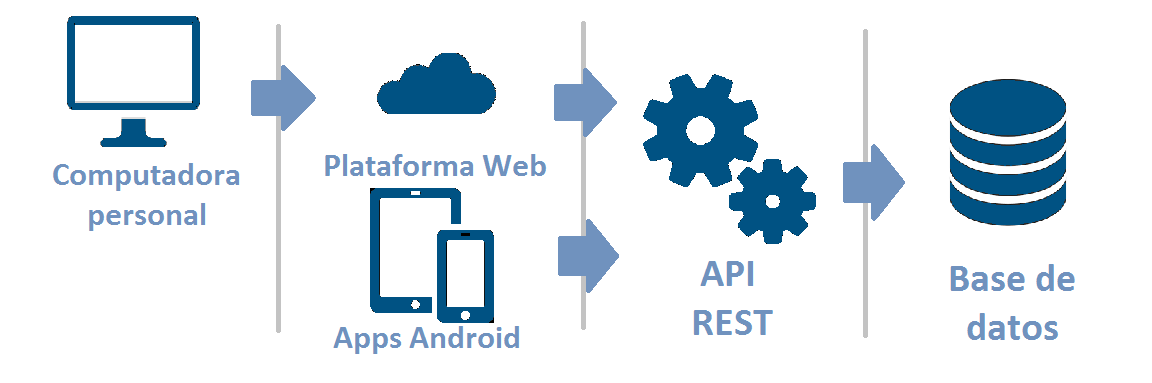
\includegraphics[scale = 0.7]{figures/proposedSystem}
	\caption{Diagrama propuesto del sistema.}
	\label{proposedSystem}
\end{figure}


\subsection*{Alcances}

El proyecto descrito en el presente documento se limita a la presentación cruda (no procesada o filtrada) de datos para el superusuario, en el registro de asistentes, miembros de staff, vendedores e inventarios para funcionar de manera integral, es decir, con interacciones entre todas las entidades descritas anteriormente.
Para el desarrollo de la API REST se utilizará el frameworkDjango REST cuya documentación y soporte se encuentran disponibles gratuitamente en línea, por lo que se evitará la generación de costos extraordinarios referentes al desarrollo de esta etapa del proyecto, pero limitando los alcances de ésta a los alcances del framework.

La API REST y la base de datos se almacenarán en servidores remotos gratuitos para evitar costos por desarrollo, despliegue, mantenimiento y consulta de ellos. Por lo tanto, el consumo de los servicios y la base de datos en sí, estarán limitados por las restricciones que conlleven dichos servidores gratuitos. Cabe aclarar que la plataforma será construida de manera escalable, y en el momento que sea requerido, estas dos entidades podrán ser trasladadas a plataformas con requerimientos y capacidades de mayor alcance.
